\chapter{Experiment}
\label{cha:exp}
In the experiment, we use the same testing data as our previous work\cite{LML}. We download audio clips from SoundJax\footnote{http://soundjax.com/}, FindSounds\footnote{http://www.findsounds.com/}, FreeSound\footnote{http://www.freesound.org} and YouTube\footnote{http://www.youtube.com/}, including sounds of events and sounds of scenes. We choose 10 scenes (bar, beach, cafeteria, church, concert, office, park, street, toilet and train) to evaluate our system. For each scene, we download 10 audio clips for testing. The length of audio clips are various from a few seconds to a few minutes. Audio clips are converted to WAVE form with single channel, 16 bits per sample point, 384kbps bit-rate.

We set the frame size to the length of 512 sample points (20ms) to extract audio features. The MFCC feature are extracted using open source code written by Klautau in 2001. The implementation is based on \cite{1163420, 237532,397093,Cardin:1993:ICM:1946943.1947011}. We combine ZCR, 12 dimensions MFCC and its $1^{st}$ and $2^{nd}$ differentials (37 dimensions in total) to train our GMM models. The number of mixtures of GMM is set to 32.


\section{Results}
Table \ref{table:ac} and Figure \ref{fig:ac} show the recognition accuracy for each audio scenes, where ``top1'' and ``top3'' refer to the number of most likely scenes taken into consideration. We obtain an average accuracy of $37\%$ for ``top1'' and $71\%$ for ``top3'' in our experiment. It shows that out system outperforms\cite{LML} a lot.

\begin{table}[htbp]
\centering
\resizebox{0.95\textwidth}{!}{
\begin{tabular}{lcccccccccc}
\toprule

      & bar & beach & cafeteria & church & concert & office & park & street & toilet & train \\
\bottomrule
top1 & $20\%$ & {\color{blue}$70\%$} & $10\%$ & $30\%$ & $20\%$ & $10\%$ & $60\%$ & $20\%$ & {\color{red}$100\%$} & $30\%$ \\
					top3 & $40\%$ & $80\%$ & $40\%$ & {\color{blue}$90\%$} & {\color{blue}$80\%$} & $30\%$ & {\color{blue}$80\%$} & {\color{red}$100\%$} & {\color{red}$100\%$} & {\color{blue}$70\%$} \\
\bottomrule
\end{tabular}
}
\caption{Recognition Accuracy for 10 Audio Scenes}
\label{table:ac}
\end{table}
\begin{figure}[!htbp]
\centering
\includegraphics[width=0.95\textwidth]{figures/comp.eps}
\caption{Recognition Accuracy for 10 Audio Scenes}
\label{fig:ac}
\end{figure}

The following confusion matrix show the result of our experiment. We can see that some of scenes have a very high recognition currency, while some of scenes are difficult to be recognized.

\begin{table}[!htbp]
\centering
\resizebox{0.95\textwidth}{!}{
\begin{tabular}{lcccccccccc}
\hline
 & bar&beach & cafeteria & church & concert & office & park & street & toilet & train\\\hline
bar & 2 & 0 & 2 & 0 & 4 & 0 & 0 & 1 & 0 & 1 \\
beach & 0 & 7 & 0 & 0 & 1 & 0 & 1 & 0 & 1 & 0 \\
cafeteria & 2 & 0 & 1 & 1 & 2 & 0 & 1 & 0 & 1 & 2 \\
church & 2 & 0 & 1 & 3 & 1 & 0 & 0 & 0 & 0 & 3 \\
concert & 2 & 0 & 2 & 1 & 2 & 0 & 1 & 0 & 0 & 2 \\
office & 0 & 2 & 2 & 0 & 1 & 1 & 0 & 0 & 3 & 1 \\
park & 0 & 1 & 2 & 0 & 0 & 0 & 6 & 0 & 1 & 0 \\
street & 0 & 0 & 1 & 0 & 1 & 0 & 1 & 2 & 0 & 5 \\
toilet & 0 & 0 & 0 & 0 & 0 & 0 & 0 & 0 & 10 & 0 \\
train & 1 & 0 & 0 & 2 & 1 & 0 & 2 & 0 & 1 & 3\\\hline
\end{tabular}
}
\caption{Confusion Matrix of 10 Scene Recognition}
\end{table}

\section{Analysis of Result}
For scenes ``bar'', ``cafeteria'', ``office'' and ``street'', there is no typical event of them in our audible event set. For example, we do not have events like copier, printer, etc. Thus the currency of these 4 scenes is low. 

Also, we find that some of noise is very similar to some events related to ``cafeteria'' and ``bar''. As the result, some of audio clips of ``concert'' and park are recognized as ``cafeteria'' or ``bar'', even if the typical events are detected, \eg dog barking in park, applause and some musical instrument sound in ``concert''.

As for ``beach'', most of the audio clips are recognized correctly. The rest of them are not recognized because {\em seabird} is not in our audible event set. The voice of {\em bird} is recognized as other events.

Moreover, the error rate is not low between ``church'' and ``train'', because the {\em train whistle} is similar to {\em chant} and some {\em music} in church.

The result of ``toilet'' is extreme good. The reason is that we can detect many audio events which rarely happen in other scene, such as {\em shower}, {\em bathtub}, etc.

